\documentclass{article}
\usepackage[utf8]{inputenc}
\usepackage{amsfonts}
\usepackage{graphicx}
\usepackage{pdfpages}
\usepackage{float}

\graphicspath{ {./figures/} }

\title{Mini Projet Data Science}
\author{HAJAGE Michael, RODRIGUES PEREIRA Lucas et PONT Mathieu}
\date{Mai 2019}

\begin{document}

\maketitle

\section{Introduction}
Dans le cadre de la première année du master informatique de l'université de Paris (anciennement Paris Descartes) il nous a été demandé dans le cours "Data Science" de réaliser un projet utilisant le jeu de données Fashion-MNIST. 

Nous devons analyser ce jeu de données à l'aide des différents algorithmes suivants:

\begin{itemize}
\item Principal Component Analysis (PCA)
\item t-distributed Stochastic Neighbor Embedding (t-SNE)
\item Autoencoder
\item K-Means
\item Support Vector Machines (SVM)
\item Linear Discriminant Analysis (LDA)
\end{itemize}

\section{Principal Component Analysis (PCA)}

Nous avons commencé par l'analyse en composantes principales dont les deux premiers axes n'expliquent que 36.49\% de la variance totale des données.

\begin{figure}[H] 
\centering
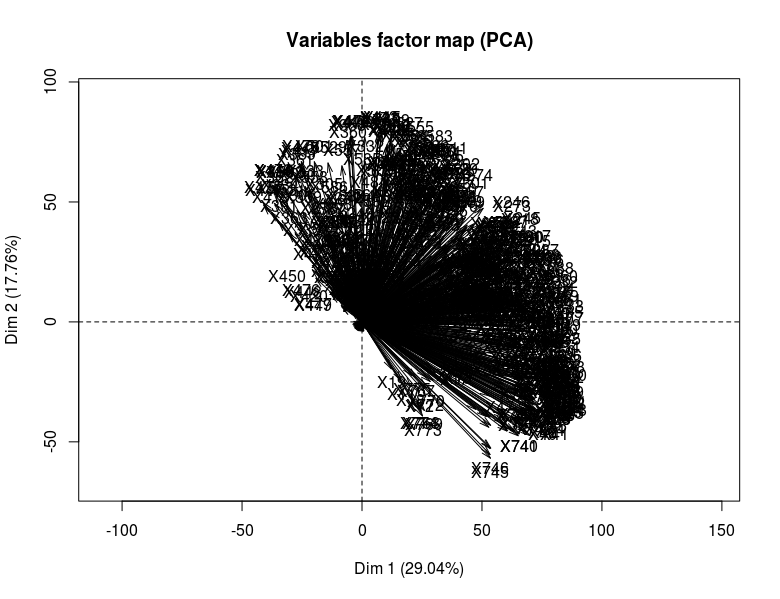
\includegraphics[width=300]{pca_var_factor_map.png}
\caption{Plan factoriel des variables avec PCA.}
\label{fig:pca_var}
\end{figure}

\begin{figure}[H] 
\centering
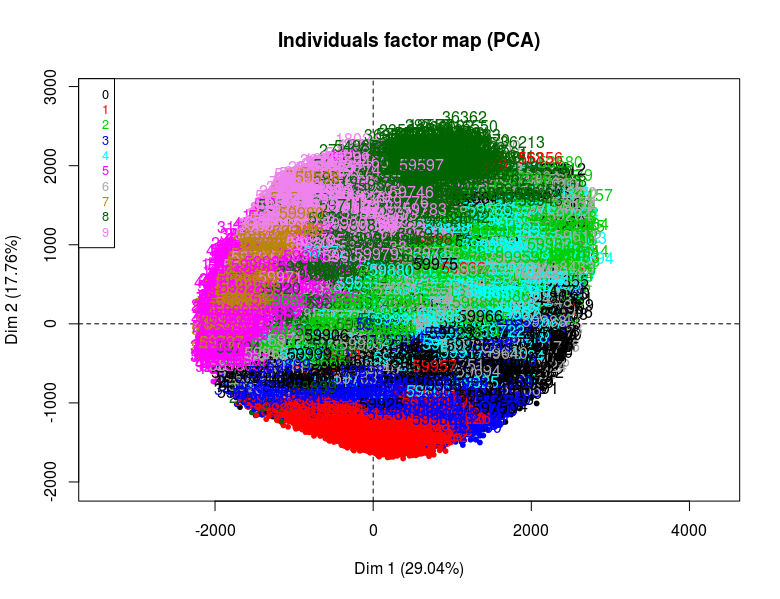
\includegraphics[width=300]{pca_ind_factor_map.png}
\caption{Plan factoriel des individus avec PCA.}
\label{fig:pca_ind}
\end{figure}

\begin{figure}[H] 
\centering
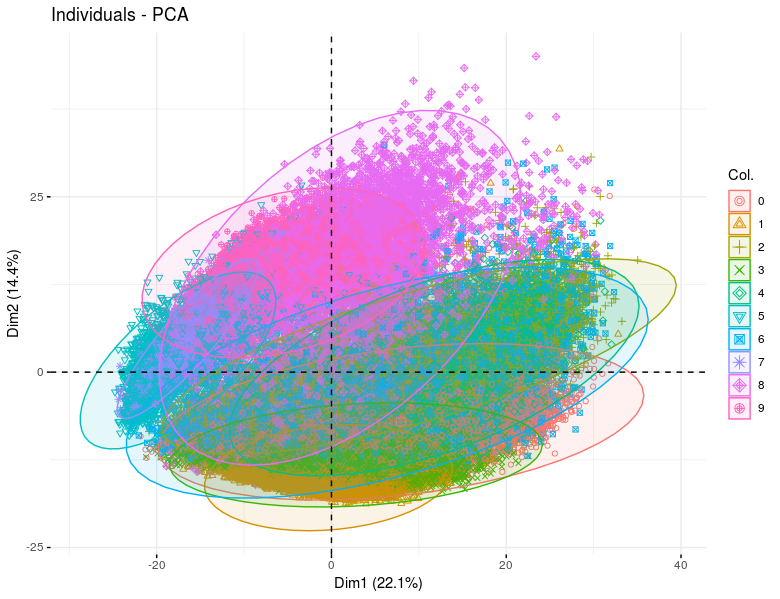
\includegraphics[width=300]{pca_ellipse.png}
\caption{Ellipse des classes avec PCA.}
\label{fig:pca_ind}
\end{figure}

\section{t-distributed Stochastic Neighbor Embedding (t-SNE)}

\section{Autoencoder}

\section{K-Means}

\section{Support Vector Machines (SVM)}

\section{Linear Discriminant Analysis (LDA)}

\section*{References}

\end{document}
